\documentclass{article}
\usepackage{graphicx} % Required for inserting images
 
\title{Mansa Trade: Connecting the world through one global payment system}

\author{
        Mansa Team \\
        team@mansa.email\\
}
\date{January 2024}

\documentclass[12pt]{article}

% \usepackage{draftwatermark}
% \SetWatermarkText{Confidential}
% \SetWatermarkScale{5}
% \SetWatermarkColor[gray]{0.95}

\usepackage{graphicx}
\usepackage{bytefield}
\usepackage{makecell}

\usepackage[]{hyperref}
\hypersetup{
    pdftitle={Mansa Trade: Connecting the world through one global payment system},
    pdfauthor={team@mansa.email},
    pdfsubject={blockchain},
    pdfkeywords={blockchain, solana, solanacash, cryptocurrency},
    bookmarksnumbered=true,
    bookmarksopen=true,
    bookmarksopenlevel=1,
    colorlinks=true,
    pdfstartview=Fit,
    pdfpagemode=UseOutlines,    % this is the option you were lookin for
    pdfpagelayout=TwoPageRight
}

\begin{document}
\maketitle

\textbf{\footnotesize Legal Disclaimer:}\scriptsize
~~Nothing in this Litepaper is an offer to sell or the solicitation of an offer to buy any tokens. Mansa Trade is publishing this Litepaper solely to receive feedback and comments from the community. If and when Mansa Trade offers for sale any tokens (or a Simple Agreement for Future Tokens), it will do so through definitive offering documents, including a disclosure document and risk factors. Those definitive documents are also expected to include an updated version of this Litepaper, which may differ significantly from the current version. If and when Mansa Trade makes such an offering in the United States, the offering likely will be available solely to accredited investors. 
Nothing in this Litepaper should be treated or read as a guarantee or promise of how Mansa Trade business or the tokens will develop or the utility or value of the tokens. This Litepaper outlines current plans, which could change at its discretion, and the success of which will depend on many factors outside Mansa Trade control, including market-based factors and factors within the data and cryptocurrency industries, among others. Any statements about future events are based solely on Mansa Trade's analysis of the issues described in this Litepaper. That analysis may prove to need to be corrected.

\begin{abstract}
Mansa Trade is a decentralized global payment system that aims to accelerate the adoption of the Solana network worldwide by adding more transaction capacity to the network.
With Solana being one of the fastest blockchains, our mission is to make the technology widely accessible to the masses through our core products by developing user-friendly mobile apps to facilitate peer a peer-to-peer payment system enabling users to send and receive funds securely with average cost per transaction of \$0.00025.
Mansa Trade focuses on cross-chain technology to bridge the gap between global financial systems through cryptocurrency by enabling multi-connectivity between Mansa Trade and various blockchains, thereby increasing interoperability all on one platform.
\end{abstract}
\newpage

\section{Decentralized Web3 P2P Platform}\normalsize
Mansa Trade Solution:
\begin{enumerate}
    \item Providing a decentralized p2p platform built on Solana blockchain.
    \item Sellers of crypto for cash only need to connect their wallets and begin trading. No KYC or account is required.
    \item All crypto is stored in a smart contract that can only be released by the depositor. Completely safe and inaccessible by a third party.
    \item Trade limits vary from 10-60 min, encouraging faster trade time between both parties.
    \item Buyers of cryptocurrency for cash have the option to KYC for more visibility, credibility, and buying power on the platform.
\end{enumerate}

\section{SolanaCash}
Mansa Trade is a Web3 decentralized peer-to-peer trading marketplace on Solana, where buyers and sellers can connect their wallets to trade crypto for cash with many different payment methods such as Cashapp, Venmo, Zelle, Wechat, Bank transfer, and more.\\

\textbf{OUR MISSION}

To bridge the gap between the global financial system and cryptocurrency by providing a platform where users are in control of how they convert crypto to fiat in a decentralized way. \\

\textbf{Features of Mansa Trade P2P D’app}
\begin{enumerate}
    \item A Web3 p2p trading platform based on smart contracts.
    \item Users are in control of their trades with no third party involved. No KYC is needed.
    \item Easily connect existing wallets to Mansa Trade d’app or mobile app. No account is needed as the wallet is the account.
    \item Embedded notification in our D'app such as SMS and email connecting web2 and web3.
    \item Wallet-to-wallet chat on the blockchain
\end{enumerate}

\section{Case Study}

\textbf{Why convert cryptocurrency to cash}

Maria is a cryptocurrency trader in the Philippines. Research shows that about 50\% of the Filipino population does not have a bank account. Every week, Maria converts her crypto into fiat. Maria usually pays about \$50 via a traditional bank or locally centralized exchange to convert crypto to cash in her local currency. Maria claims it takes about 3 business days to get fiat into her bank account. Maria also needs to create an account and take part in a mandatory KYC with a government-issued ID.\\

\textbf{Solution}

Maria now uses the Mansa Trade P2P platform to connect her crypto wallet directly to our D’app and selects from our list of available offers and vendors that accept her payment methods. She uses G-Cash as her preferred payment method. Maria creates a sell order and deposits crypto into the smart contract. The vendor gets notified and sends fiat to Maria in her local currency using her preferred payment method. Maria is able to convert crypto to cash in less than 30 minutes with relatively low transaction fees. Maria is also able to communicate with the vendors via our platform messaging system. All of Maria’s data is stored securely on the blockchain. Maria can access her order history by connecting her wallet to Mansa Trade P2P d’app.

\section{Target Market and Potential}

Asia has had the biggest continent economy since 2010, accounting for 39\%-47\% of the world economy, according to Statistics Times. This is equivalent to \$68.7 trillion, two times the second-ranked continent Europe.

With this massive economy, 70\% of the population is unbanked. Governments across Asia mitigated this problem by introducing mobile wallets since smartphone is prevalent in Asia. With approximately 60\%-75\% of the population owning a smartphone, the unbanked population is now estimated at around 30\%-40\%.

Tapping this market has more upside potential than risk. Asia has no clear regulation on peer-to-peer market exchange. Crypto regulation is also in its infancy, while some advanced economies governments such as South Korea and Japan have some regulatory measures for crypto central exchanges with no mention of peer-to-peer exchange. 

In retrospect, low regulatory risk, low downside risk, and high growth potential. According to coindesk.com, active wallets for Solana network increased by 58\% in 2022. New users peaked at over 400,000 in May 2022 before gradually declining to 240,000. This is despite s market-wide price decline.\\

\textbf{Key Binance Statistics:}

Binance has one of the biggest p2p platforms, having 28 million users on its platform in 2021 and reaching a 24-hour trading volume of 76 billion dollars. 
Assuming we capture a few \% of this market from both Solana and Binance, the projected 5-year YoY growth is demonstrated in the table below.

\begin{table}[h]
    \centering
    \begin{tabular}{|c|c|c|c|c|} \hline 
         Year&  Actual Users&  Target Users&  Achieved \%& YoY \%\\ \hline 
         2023&  1 000&  1 000&  100& 10\\ \hline 
         2024&  10 000&  100 000&  10& 1\\ \hline 
         2025&  1 000 000&  1 000 000&  100& 50\\ \hline 
         2026&  2 000 000&  3 000 000&  66.6& 40\\ \hline 
         2027&  5 000 000&   6 000 000&  83.3& 50\\ \hline
    \end{tabular}
    
    
\end{table}


\section{Business Plan and Model}

\textbf{Projected Revenue Based on Fees}

Revenue is calculated based on total dollar value of transactions processed and completed on the platform.


\textbf{Estimated 5-year Revenue Stream (YoY)}

Dollar Value of Transactions Volume: 

Platform Fees Per Trade: Buyers 0.1\% and Sellers 0.2\%

Estimated Trade per user: \$100/month


\begin{table}[h]
    \centering
    \begin{tabular}{|c|c|c|c|} \hline 
         Year&  Actual Users&  Total Volume& Revenue \$\\ \hline 
         2023&  1 000&  1 200 000& 3 600\\ \hline 
         2024&  100 000&  12 000 000& 36 000\\ \hline 
         2025&  1 000 000&  1 200 000 000& 3 600 000\\ \hline 
         2026&  3 000 000&  2 400 000 000& 7 200 000\\ \hline 
         2027&  6 000 000&  6 000 000 000& 18 000 000\\ \hline
    \end{tabular}
    
    
\end{table}

\textbf{How?}

\begin{enumerate}
    \item Decentralized peer-to-peer exchange.
    \item No third party is involved; everything on our platform is smart contract-based.
    \item No KYC for 90\% of platform users.
    \item Extremely low trading fees: We charge Sellers 0.2\% and Buyers 0.1\% per trade.
    \item Uphold the self-custody of the user's asset.
    \item Multi-network platform.
\end{enumerate}

\textbf{Below is our planned development}

\begin{figure}[h]
  \begin{center}
    \centering
    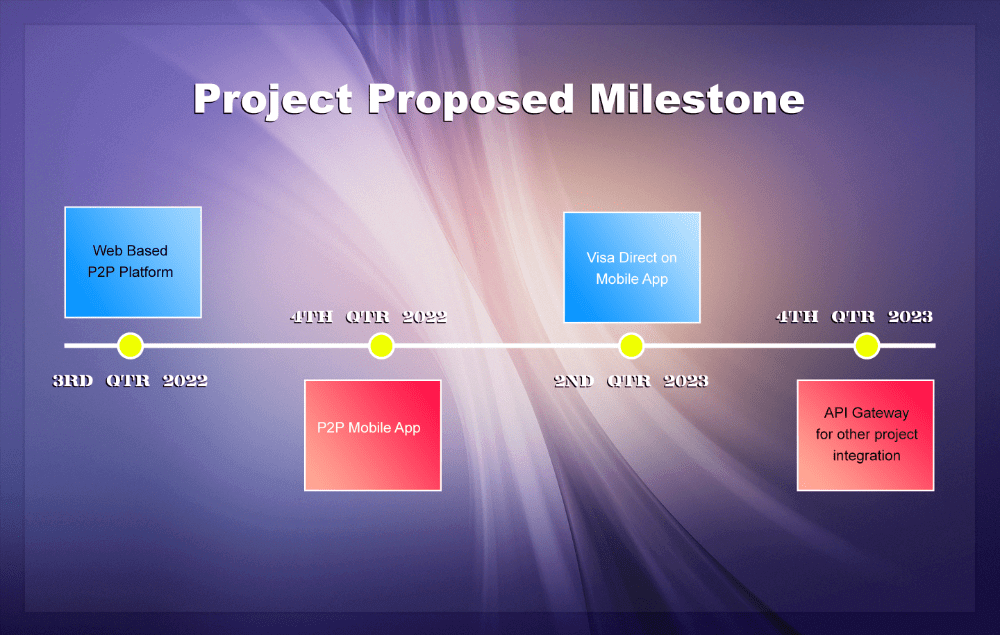
\includegraphics[width=0.9\textwidth]{fig/planned_dev.png}
    \caption[Fig 1]{Proposed Milestone\label{fig:poh_insert}}
  \end{center}
\end{figure}

\begin{enumerate}
    \item Currently, our P2P platform is in beta testing. Development began in June 2022 and is currently around 95\% completed. Currently working on improvements, bugs, and updating the platform for better user experience. The platform is available in 7 different languages. We will start marketing once we debug the platform and launch on the mainnet.
    \item We started the development of the P2P mobile app of the P2P d'app. The app would be available for IOS and Android.
    \item Because of the extremely decentralized nature of the Mansa Trade P2P platform, Visa Direct was supposed to be implemented as part of the payment methods. However, Visa Direct is heavily centralized, and working with 3rd party provider takes a lot of time and legal documents. Nevertheless, Visa Direct will be added to the list of payment methods to use outside the platform. Users can use this as a payment gateway for P2P users as well as send fiat to fiat to any Visa account.
    \item API development for crypto project adaption: API for the platform would be free and open source. Projects would be able to sell directly in their own gaming or DeFi platform using our P2P API. They would be able to host payment and P2P exchange on their own server mirroring what we have exactly in our official site with full function.
\end{enumerate}

\textbf{5-yr Growth Projection}

\begin{figure}[h]
  \begin{center}
    \centering
    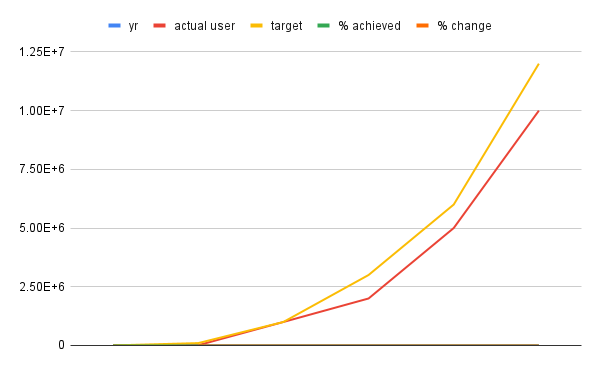
\includegraphics[width=0.9\textwidth]{fig/5y-grow-projection.png}
    \caption[Fig 2]{5-yr Growth Projection\label{fig:poh_insert}}
  \end{center}
\end{figure}

\section{Existing Alternatives}

\begin{figure}[h]
  \begin{center}
    \centering
    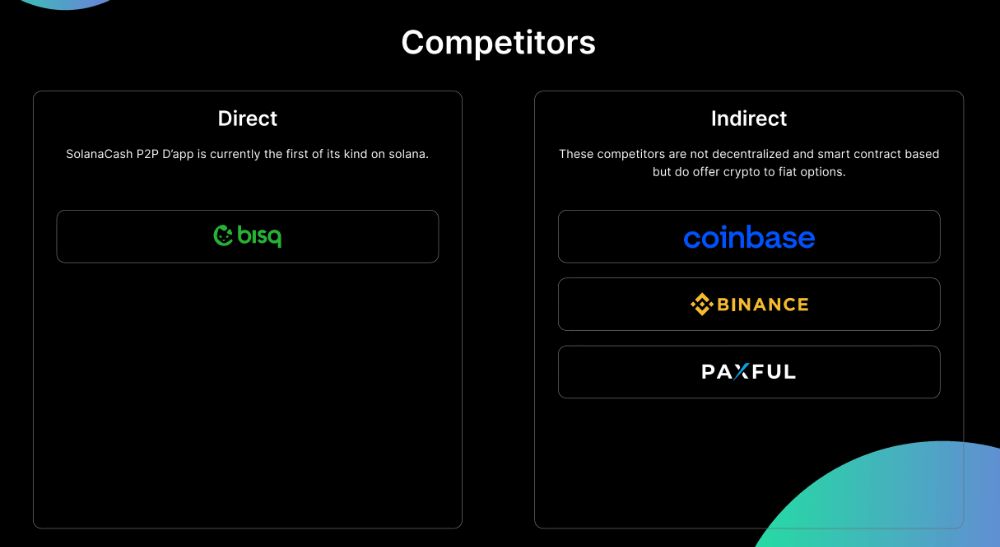
\includegraphics[width=0.9\textwidth]{fig/alts.png}
    \caption[Fig 3]{Direct and Indirect Competitors\label{fig:poh_insert}}
  \end{center}
\end{figure}

\textbf{Direct and Indirect Competitors}

Peer-to-peer exchange is not new; this is as old as barter trade, which is still being practiced in Asia and some parts of the world. This is the growth driver for most CEX in the crypto industry. P2P serves as onramp and off ramp tool for these CEXes giving them high volume turnout.

Mansa Trade P2P is easy to understand and use compared to traditional banking system which takes approximately 3 banking days using the swift system and cost \$25 USD fee for sender and receiver. This is not ideal for small amount transfer nor small traders trying to make it in crypto. Mansa Trade charges very low fees per trade as compared to most of our competitors. Our fees vary from 0.1-0.2\% per trade.

\end{document}
This is never printed